\chapter{Demand Response}
\label{chp:dr}

\glsresetall

\section{Summary}

Large consumers can participate in \textit{\acrlong{DR}} to receive financial rewards by reducing consumption at times with high electricity wholesale prices.
One way to earn rewards without changing existing consumption patterns is to use batteries.
We can charge batteries during times with low prices and discharge them at times with high prices.
This work develops a scheduling algorithm that decides the best times to charge and discharge batteries, in order to maximise the rewards.
This algorithm combines \acrlong{LP} and \acrlong{RHRS} to use demand and price forecasts for scheduling while considering uncertainty in these forecasts. 
Further works are still required to evaluate the results of this algorithm. 


\section{Demand Response Financial Rewards}
\label{dr:rewards}

\Gls{DR} refers to activities of reducing loads in response to financial incentives. 
Monash receives financial rewards for reducing loads when the wholesale price is above a threshold via contracts with the retailer. Monash will retain 60\% of the wholesale price above this trigger price for load reduction delivered beyond the adjusted baseline load, with the retailer retaining the other 40\%. 
Several conditions are required for Monash to meet, in order to receive financial rewards from \gls{DR}, including:
\begin{itemize}
	\item Meeting trigger price: Load reductions should occur when the wholesale price is above the trigger price, which is currently defined at \$300 / MWh for the Clayton campus.
	
	\item Meeting the minimum load reduction: Monash should reduce at least 1 kWh of the loads in order to receive rewards. 
	%todo: 1kW or 1kWh ?
	
	\item Defining the load measurements: The loads should be measured at 15-minute intervals, however, the load reductions are calculated based on the 30-minute averages. 
	
\end{itemize}

\subsection{Calculation of Financial Rewards}
\label{dr:rewards:rewards}

The financial reward is calculated for each trading interval where the \gls{DR} conditions are met. The duration of a trading interval was thirty (30) minutes before Oct 2021, however, is now five (5) minutes. In respect to a trading interval $n$, the load reduction financial benefit is based on the wholesale spot price, the adjusted baseline load, the measured or the actual load, a \textit{\gls{LRV}} and a loss factor, described as Equation~\ref{equ:dr:reward}. 

\begin{equation}
	\label{equ:dr:reward}
	\forall n, ~ \gls{reward_n}	= \gls{spot_price_n} \times min(0,  ( \gls{baseline_load_n} - \gls{actual_load_n} )) \times \gls{LRV} \times Loss factor
\end{equation}
where:
\begin{itemize}
	\item \gls{reward_n} is the reward for the trading interval $n$,
	
	\item \gls{spot_price_n} is the wholesale spot price for the trading interval $n$,
	
	\item \gls{baseline_load_n} is the baseline load for the trading interval $n$ in MWh,
	
	\item \gls{actual_load_n} is the measured or the actual load for the trading interval $n$ in MWh,
	
\end{itemize}
The wholesale spot prices are provided by \gls{AEMO}. The actual loads are measured by electricity meters. The \gls{LRV} is set to be 60\% for Monash. The loss factor is a fixed value (about 0.9) that applies to the specified NMI (ID: VEEE08KH3V), which is neglect-able in this work. The adjusted baseline load needs to be calculated from historical loads. 

\subsection{Calculation of Baseline Loads}
\label{dr:rewards:baseline}

The baseline load with the respect to a specified NMI and a trading interval is calculated using:

\begin{itemize}
	\item The average amount, in MWh, of the measured load (with respect to the specified NMI) for the ten (10) trading intervals occurring at the same time of day as that trading interval on the ten (10) like days immediately preceding on which that trading interval occurs;
	
	\item The relevant uplift factor for the corresponding maximum temperature of the day. 
\end{itemize}


The baseline load for a trading interval of a day is calculated from the loads of the same trading interval in the prior ten like days and a uplift factor that corresponds to the maximum temperature of the day. 


\subsubsection{Like days}
\label{dr:like-days}

%The baseline load for a trading interval of a day is calculated from the loads of the same interval in the prior ten like-days. 
A like day is defined as follows:

\begin{itemize}
	\item With respect to a trading interval occurring on a Monash work day, a like day should be a Monash work day.
	
	\item With respect to a trading interval occurring on a non Monash work day, a like day should be a non Monash work day. For example, if an interval on a Saturday has a spot price greater than the trigger price \$300 / MWh, then the baseline is set using the former five (5) Saturdays and five (5) Sundays (ten days total) assuming no public holidays occurred in that period.
	
	\item Like days exclude any day on which \textbf{any} trading interval has occurred with respect to which a payment needs to be made. For example, if a \gls{DR} load reduction event has occurred in any interval on one of the prior ten (10) like-days that would ordinarily be used to calculate a baseline, and Monash successfully actioned a load reduction such that the retailer was subject to making a payment for that interval on that day, then \textbf{that whole day} is excluded from the baseline, and the next prior like-day needs to be used to set the respective baseline.
	
\end{itemize}
The definition of Monash work days is provided in \url{https://www.monash.edu/students/admin/dates/holidays}.

\subsubsection{Uplift Factor}

The uplift factors corresponding to maximum temperatures are listed as Table~\ref{dr:intro:uplift}. 

\begin{table}[ph]
	\caption{Uplift factors for maximum temperature values}
		\label{dr:intro:uplift}
\begin{tabularx} {\linewidth} {Y Y}
	\toprule
	\textbf{Maximum Temperature} & \textbf{Uplift Factor} \\
	\midrule
	27 & 106\% \\
%	\hline
	28 & 106\% \\
%	\hline
	29 & 106\% \\
%	\hline
	30 & 116\% \\
%	\hline
	31 & 116\% \\
%	\hline
	32 & 116\% \\
%	\hline
	33 & 116\% \\
%	\hline
	34 & 122\% \\
%	\hline
	35 & 122\% \\
%	\hline
	36 & 122\% \\
%	\hline
	37 & 122\% \\
%	\hline
	38 & 127\% \\
%	\hline
	39 & 127\% \\
%	\hline
	40 & 127\% \\
%	\hline
	$\geq$ 40 & 127\% \\
	\bottomrule
	
\end{tabularx}
\end{table}


\section{Methodology of Battery Scheduling for Demand Response}

We can use \glspl{battery} to discharge during intervals with wholesale prices that are higher than the trigger price, and charge outside those periods, in order to earn financial rewards without changing the existing consumption patterns. 

Similar to the method developed in Chapter~\ref{chp:pdm}, the work in this chapter follows the methodology explained in Section~\ref{intro:methodology}. More specifically, this work combines \textit{\glsfirst{LP}} models and \textit{\glsfirst{RHRS}} to optimally schedule batteries and incorporate uncertainty in demand and price forecasts. 

%schedules \glspl{battery} using optimisation algorithms based on demand and price forecasts. More specifically, this work follows the methodology introduction in Section~\ref{intro:methodology}, which is combing \textit{\glsfirst{LP}} models and \textit{\glsfirst{RHRS}} to optimally schedule batteries and incorporate uncertainty in the demand forecasts. 


%\subsection{Chapter Structure}
%
%This chapter presents the development of the battery scheduling algorithm for peak demands management as follows: 
%\begin{itemize}
%	\item Section~\ref{dr:prob} presents the mathematical notations and formulation of the battery scheduling problem for \gls{DR}. 
%	
%	\item Section~\ref{dr:method} introduces the \gls{LP} model for solving the battery scheduling problem and the \gls{RHRS} for incorporating uncertainty in demand forecasts. 
%	
%	\item Section~\ref{dr:exp}:
%	
%	\item Section~\ref{dr:conclusion}:
%	
%\end{itemize}

\section{Battery Scheduling Problem for Demand Response}
\label{dr:prob}

This work studies a battery scheduling problem where batteries are scheduled to maximise the financial rewards from \gls{DR}. 
This section presents the input parameters, variables, constraints, objective functions and mathematical formulation of the battery scheduling problem. 

\subsection{Problem Parameters}

The input parameters for this battery scheduling problem include time intervals, battery specifications, parameters related to demand response rewards, load forecasts, historic loads, price forecasts, historic prices and objective weights. 

\subsubsection{Time Interval}

A day is considered as a finite number of time intervals for scheduling. 
%At the time of this work, the wholesale electricity price is provided by \gls{AEMO} for every thirty minutes. Therefore, this work divides a day into 48 thirty-minute intervals for scheduling batteries. 
We assume that the charge or discharge rate of a battery does not change in a time interval. Let us write:

\begin{itemize}
	\item \gls{T} as the length in minutes of each time interval,
	
	\item $\gls{N^day} = 1440 / \gls{T}$ as the total number of time intervals per day,
	
	\item $\gls{N^hour} = 60 / \gls{T} $ as the total number of time intervals per hour,
	
	%	\item \gls{n} as the index of a time interval.
\end{itemize}
We have chosen $\gls{T} = 30 $ mins for this work, because at the time of this work, the wholesale electricity prices are updated every thirty minutes. 

\subsubsection{Battery Specification}

The total number of batteries is denoted as \gls{N^battery}. Each battery $i \in [1, \gls{N^battery}]$ is modelled by the following elements:

\begin{itemize}
	\item \gls{init_energy}: the initial energy level at the beginning of the day (in kWh)
	
	\item \gls{min_cap}: the minimum allowed energy capacity (in kWh)
	
	\item \gls{max_cap}: the maximum allowed energy capacity (in kWh)
	
	\item \gls{max_power}: the maximum power rate (in kW)
	
	\item \gls{ch_bn}: the amount of power charged to the battery at time step $n$ (in kW): 
	
	\item \gls{disch_bn}: the amount of power discharged from the battery at time step $n$ (in kW) 
	
	\item \gls{rte}: the round-trip efficiency (between 0 and 1)
	
	\item \gls{soc_n}: a \gls{SOC} profile --- the amount of energy remaining in the battery at time step $n$ (in kWh)
\end{itemize}


\subsubsection{Demand Response Reward Parameters}

The parameters required for calculating the demand response rewards include:

\begin{itemize}
	\item Trigger price \gls{trigger_price}: An essential condition for receiving the demand response rewards, as explained in Section~\ref{dr:rewards}.
	
	\item Forecast maximum temperature: The maximum temperature forecasted at the time of the demand forecast. 
	
	\item Uplift factors \gls{alpha_uplift}: The uplift factor associated with the maximum forecasted temperature for scaling the baseline loads, as explained in Section~\ref{dr:rewards:baseline}.
	
	\item Load reduction value \gls{LRV}: A value set for Monash, as explained in Section~\ref{dr:rewards:rewards}.
	
	\item Loss factor: A factor specific to the electricity meter used for measuring the actual loads, as explained in Section~\ref{dr:rewards:rewards}. 
\end{itemize}

In addition, we have introduced binary variables that indicate the time intervals whose forecast spot prices are above the trigger price. Theses binary variables are defined as $\gls{t_dr} = \{ \glssymbol{t_dr} = 1~ if ~ \gls{spot_price_n} \geq \gls{trigger_price} ~ else~ 0~ \vert ~ n \in [1,\gls{N^day}] \}$.

 
\subsubsection{Load Forecast}

Load forecasts are required to plan the battery operations in advance. 
At the time of this work, at each time interval $n$, the demand is forecasted from the upcoming time interval $n+1$ until 6pm of the same day. However, to allow batteries to charge after 6pm, we assume the forecasted demand after 6pm is zero. Let us write \gls{load} as the load per time interval in kWh. 

%The load data required for this work is the load forecast \gls{load} for each time step $n$ (in kWh). 

\subsubsection{Historic Load}

Historic loads are used for calculating the baseline loads from like-days. Ideally, at each time interval $n$, the historic loads should be for the three months prior to the current time interval. If less than three months of data is provided, the baseline loads will be calculated from the available data only. Let us write the historic loads at time interval $n$ of day $d$ as \gls{historic_load_n}.

\subsubsection{Price Forecast}

Price forecasts are required to prepare batteries for potential demand response opportunities. The price forecasts are provided by \gls{AEMO}. Let us write \gls{forecast_price_n} as the forecasted spot price per time interval in \$/MWh. 
%At the time of this work, at each time interval $n$, the demand is forecasted from the upcoming time interval $n+1$ until 6pm of the same day. However, to allow batteries to charge after 6pm, we assume the forecasted demand after 6pm is zero. Let us write \gls{demand} as the demand per time interval in kW. 

\subsubsection{Historic Price}

Historic prices are used for identifying past demand response event days, and excluding those days from like days for calculating baseline demands. Let us write \gls{historic_price_n} as the historic spot price per time interval in \$/MWh of day $d$. 

\subsubsection{Objective Weight}

This work has considered multiple objectives including maximisation of the financial reward and minimisation of a penalty cost of charging or discharging batteries frequently. The penalty cost is introduced to prevent batteries from fluctuating between charging and discharging during the day. 
%The impacts of this penalty will be demonstrated in more details in Section~\ref{exp}. 
The objective weights are denoted as:

\begin{itemize}
	\item The weight of the financial reward: \gls{w_reward}.
	
	\item The weight of the penalty cost: \gls{w_penalty}.
\end{itemize}


\subsection{Problem Variables}

The decision variables include the amount of power charged to or discharged from each battery at each time interval: \gls{ch_bn} and \gls{disch_bn}.


\subsection{Problem Constraints}

The constraints are the same as those in Section~\ref{pdm:problem:contraints} in Chapter~\ref{chp:pdm}.

\subsection{Problem Objectives}

The objectives of our battery scheduling problem for demand response include maximisation of the financial reward and minimisation of a penalty cost of charging or discharging batteries frequently. The penalty cost \gls{g_battery} is the same as that in Section~\ref{pdm:problem:objectives}. The financial reward objective is calculated as Equation~\ref{equ:dr:reward}. The combined objective \gls{h_combined} for demand response is described as

\begin{equation}
	\label{dr:problem:obj}
	\gls{h_combined} = \gls{w_reward} \times \sum_{n=1}^{\gls{N^day}} \gls{reward_n} \times \glssymbol{t_dr} + \gls{w_penalty} \times \gls{g_battery}
\end{equation}


\subsection{Formal Problem Formulation}

The battery scheduling problem for demand response can be formulated as follows:
%This problem seeks the best values for the charge/discharge per time step: \gls{ch_bn} and \gls{disch_bn} that solves the following problem:

\begin{equation*}
	\label{dr:problem:formulation}
	\begin{aligned}
		& {\textsf{minimise}}
		& &  \gls{h_combined}   \\
		& \textsf{subject to}
		& & 
		(\ref{constraint:either-charge-discharge}), 
		~(\ref{constraint:max-charge}), 
		~(\ref{constraint:max-discharge}), 
		~(\ref{constraint:min-max-cap}), 
		~(\ref{constraint:init-energy}), 
		%		~(\ref{constraint:end-energy}), 
		~(\ref{constraint:soc})\\
	\end{aligned}
\end{equation*}

\section{Battery Scheduling Method for Demand Response}
\label{dr:method}

Same as the solution presented in Section~\ref{pdm:method} of Chapter~\ref{chp:pdm}, the solution to battery scheduling for demand response uses a \glsfirst{LP} model and a \glsfirst{RHRS}. The details of \gls{RHRS} has been presented in Section~\ref{pdm:method}.  This section focuses on the algorithm for calculating the baseline loads in Section~\ref{dr:method:baseline} and the \gls{LP} model for maximising demand response rewards in Section~\ref{dr:method:model}. 

\subsection{Baseline Load Calculation}
\label{dr:method:baseline}

Currently the baseline load is calculated using historic loads only without historic prices, due to the absence of sufficient historic prices for testing. This means, past \gls{DR} event days are not excluded. 

\begin{algorithm}[tbh]
		\caption{Calculation of Baseline Loads}
		\label{single:alg:ogs} 
		\begin{algorithmic}[1]
		
				\Require Historic loads %and historic prices
				
				\ForAll{time interval $n$ in the scheduliung horizon}
				
					\State Identify like days using the conditions introduced in Section~\ref{dr:like-days}. 
					
					\State  Sum up the loads at the same interval of the past ten like days. 
					
					\State Calculate the average load of the ten like days at time interval $n$. 
				
				\EndFor
							
				\Ensure The average load per time interval in the scheduling horizon. 
			\end{algorithmic}
	\end{algorithm}

\subsection{Linear Programming Model for Demand Response}
\label{dr:method:model}

\begin{figure}[hp!]
	\centering
	\caption{\gls{LP} model for solving our battery scheduling problem for demand response}
	\label{dr:method:lp}
	% ======== MIP model for the DSP-SH ========== %
	\begin{lstlisting}[language=minizinc,escapeinside={(*@}{@*)}]
% ---------- Input parameters ---------- % (*@\label{mzn:lp:dr:paramStart}@*) 		
int: num_intervals; 			(*@\label{mzn:lp:dr:num_intervals}@*)
int: num_intervals_hour;    (*@\label{mzn:lp:dr:num_intervals_hour}@*)
int: eod_interval; 				(*@\label{mzn:lp:dr:eod_interval}@*) 
set of int: INTERVALS = 1..num_intervals; 

int: num_batteries;
set of int: BATTERIES = 1..num_batteries;			(*@\label{mzn:lp:dr:num_batteries}@*)
array[BATTERIES] of float: init_socs;   	  	    	  (*@\label{mzn:lp:dr:init_socs}@*)
array[BATTERIES] of float: min_socs;   					(*@\label{mzn:lp:dr:min_socs}@*)
array[BATTERIES] of float: max_socs;   				   (*@\label{mzn:lp:dr:max_socs}@*)
array[BATTERIES] of float: max_powers;   	 	   (*@\label{mzn:lp:dr:max_powers}@*)
float: power_limit = max(max_powers);			
array[BATTERIES] of float: efficiencies;				(*@\label{mzn:lp:dr:efficiencies}@*)

array[INTERVALS] of float: forecast_loads;					(*@\label{mzn:lp:dr:forecast_loads}@*)
float: load_limit;
array[INTERVALS] of float: baseline_loads;    (*@\label{mzn:lp:dr:baseline_loads}@*)
array[INTERVALS] of float: forecast_prices;          (*@\label{mzn:lp:dr:forecast_prices}@*)

% dr charges
float: load_reduction_value;							     (*@\label{mzn:lp:dr:lrv}@*)
float: loss_factor;													  (*@\label{mzn:lp:dr:loss_factor}@*)
float: w_penalty; (*@\label{mzn:lp:dr:w_penalty}@*) 
float: w_eod; (*@\label{mzn:lp:dr:w_eod}@*) 	(*@\label{mzn:lp:dr:paramEnd}@*)

% ---------- Variables ---------- % (*@\label{mzn:lp:dr:varsStart}@*)
array[BATTERIES, INTERVALS] of var 0..power_limit: charges;        (*@\label{mzn:lp:dr:charges}@*)
array[BATTERIES, INTERVALS] of var -power_limit..0: discharges;  (*@\label{mzn:lp:dr:discharges}@*)
array[BATTERIES, INTERVALS] of var float: soc;								 (*@\label{mzn:lp:dr:socs}@*)
array[INTERVALS] of var 0..demand_limit: modified_loads = array1d([forecast_loads[i] + sum(b in BATTERIES)(charges[b, i] + discharges[b, i])| i in INTERVALS]);  (*@\label{mzn:lp:dr:modified_loads}@*) (*@\label{mzn:lp:dr:varsEnd}@*)
		
% ---------- Constraints ---------- %	(*@\label{mzn:lp:dr:ctsStart}@*)
% Charge or discharge only constraint   (*@\label{mzn:lp:dr:charge-discharge_cts}@*)
constraint forall(b in BATTERIES, i in INTERVALS)(charges[b, i] * discharges[b, i] = 0); 
		
% Maximum power constraints  (*@\label{mzn:lp:dr:power_cts}@*)
constraint forall(b in BATTERIES, i in INTERVALS)(discharges[b, i] <= 0.0);
constraint forall(b in BATTERIES, i in INTERVALS)(discharges[b, i] >= -max_powers[b]);
		
constraint forall(b in BATTERIES, i in INTERVALS)(charges[b, i] >= 0.0);
constraint forall(b in BATTERIES, i in INTERVALS)(charges[b, i] <= max_powers[b]);
		
% Maximum-minmum capacity constraints  (*@\label{mzn:lp:dr:max-min-cap_cts}@*)
constraint forall(b in BATTERIES, i in INTERVALS)(soc[b, i] <= max_socs[b]);
constraint forall(b in BATTERIES, i in INTERVALS)(soc[b, i] >= min_socs[b]);

% SOC constraints   (*@\label{mzn:lp:dr:soc_cts}@*)
constraint forall(b in BATTERIES) 
(soc[b, 1] * num_intervals_hour - init_socs[b] * num_intervals_hour = 
charges[b, 1] * efficiencies[b] + discharges[b, 1]);

constraint forall(b in BATTERIES, i in 2..num_intervals) 
(soc[b, i] * num_intervals_hour - soc[b, i - 1] * num_intervals_hour = 
charges[b, i] * efficiencies[b] + discharges[b, i]); (*@\label{mzn:lp:dr:ctsEnd}@*)

% ---------- Objectives ---------- % (*@\label{mzn:lp:dr:objStart}@*)
var float: eod_penalty = sum(i in INTERVALS, r in RATES, b in BATTERIES) ((max_socs[b] - soc[b, i]) * (1 - charge_times[r, i])); (*@\label{mzn:lp:dr:eod_penalty}@*)
var float: penalty = sum(b in BATTERIES, i in INTERVALS)(charges[b, i]); (*@\label{mzn:lp:dr:penalty}@*)
var float: returns = - sum(i in INTERVALS)
(forecast_prices[i] * load_reduction_value * loss_factor *
(baseline_loads[i] - modified_loads[i])); (*@\label{mzn:lp:dr:returns}@*)
var float: combined_obj = costs + penalty * w_penalty + eod_penalty * w_eod; (*@\label{mzn:lp:dr:combined_obj}@*) (*@\label{mzn:lp:dr:objEnd}@*)
solve minimize combined_obj;
\end{lstlisting}
\end{figure}

Figure~\ref{dr:method:lp} shows the \gls{LP} model for solving the battery scheduling problem for demand response. We declare the input parameters from Line~\ref{mzn:lp:dr:paramStart} to~\ref{mzn:lp:dr:paramEnd}, including:
\begin{itemize}
	\item The number of time intervals per day: \mzninline|num_intervals|, line~\ref{mzn:lp:dr:num_intervals},
	
	\item The number of time intervals per hour: \mzninline|num_intervals_hour|, line~\ref{mzn:lp:dr:num_intervals_hour},
	
	\item The index of the last time interval of the day: \mzninline|eod_interval|, line~\ref{mzn:lp:dr:eod_interval},
	
	\item The number of batteries: \mzninline|num_batteries|, line~\ref{mzn:lp:dr:num_batteries},
	
	\item The initial \glspl{SOC} or energy levels: \mzninline|init_socs|, line~\ref{mzn:lp:dr:init_socs},
	
	\item The minimum \glspl{SOC} or capacities: \mzninline|min_socs|, line~\ref{mzn:lp:dr:min_socs},
	
	\item The maximum \glspl{SOC} or capacities: \mzninline|max_socs|, line~\ref{mzn:lp:dr:max_socs},
	
	\item The maximum power rates: \mzninline|max_powers|, line~\ref{mzn:lp:dr:max_powers},
	
	\item The battery efficiencies: \mzninline|efficiencies|, line~\ref{mzn:lp:dr:efficiencies},
	
	\item The load forecast: \mzninline|forecast_loads|, line~\ref{mzn:lp:dr:forecast_loads},
	
	\item The baseline loads: \mzninline|baseline_loads|, line~\ref{mzn:lp:dr:baseline_loads},
	
	\item The price forecast: \mzninline|forecast_prices|, line~\ref{mzn:lp:dr:forecast_prices},
	
	\item The load reduction value: \mzninline|load_reduction_value|, line~\ref{mzn:lp:dr:lrv},
	
	\item The loss factor: \mzninline|loss_factor|, line~\ref{mzn:lp:dr:loss_factor},
	
	\item The weight for the penalty cost of charging/discharging \glspl{battery} frequently: \mzninline|w_penalty|, line~\ref{mzn:lp:dr:w_penalty}.
	
	\item The weight of the penalty cost of not fully charging \glspl{battery} before the end of the day: \mzninline|w_eod|, line~\ref{mzn:lp:dr:w_eod}.
\end{itemize}

We introduce the variables from line~\ref{mzn:lp:dr:varsStart} to line~\ref{mzn:lp:dr:varsEnd}, including:
\begin{itemize}
	
	\item The amount of power charged to each battery per time interval: \mzninline|charges|, line~\ref{mzn:lp:dr:charges}.
	
	\item The amount of power discharged from each battery per time interval: \mzninline|discharges|, line~\ref{mzn:lp:dr:discharges}.
	
	\item The \gls{SOC} of each battery per time interval: \mzninline|socs|, line~\ref{mzn:lp:dr:socs}.
	
	\item The modified load per time interval: \mzninline|modified_loads|, line~\ref{mzn:lp:dr:modified_loads}.
\end{itemize}

We define the constraints from line~\ref{mzn:lp:dr:ctsStart} to line~\ref{mzn:lp:dr:ctsEnd}, including:
\begin{itemize}
	\item The \textit{charge or discharge only constraint}: line~\ref{mzn:lp:dr:charge-discharge_cts}.
	
	\item The \textit{maximum power constraint}: line~\ref{mzn:lp:dr:power_cts}.
	
	\item The \textit{maximum-minimum capacity constraint}: line~\ref{mzn:lp:dr:max-min-cap_cts}.
	
	\item The \textit{\gls{SOC} constraints}: line~\ref{mzn:lp:dr:soc_cts}.
	
\end{itemize}

We specify the objective functions from line~\ref{mzn:lp:dr:objStart} to line~\ref{mzn:lp:dr:objEnd}, including:
\begin{itemize}
	
	\item The penalty cost of not fully charging \glspl{battery} before the end of the day: \mzninline|penalty|, line~\ref{mzn:lp:dr:penalty}.
	
	\item The penalty cost of charging/discharging \glspl{battery} frequently: \mzninline|penalty|, line~\ref{mzn:lp:dr:penalty}.
	
	\item The financial rewards: \mzninline|returns|, line~\ref{mzn:lp:dr:returns}.
	
	\item The combined objective: \mzninline|combined_obj|, line~\ref{mzn:lp:dr:combined_obj}.
\end{itemize}

Note that the trigger price needs to be multiplied by 1000 if it is in \$ / MWh, because the loads and the battery charges/discharges are in kWh or kW. 


\section{Experimental Results of Battery Scheduling Method for Demand Response}

This section presents the experiment environments, steps and results that demonstrate the effectiveness of our battery scheduling method for demand response. 

\subsection{Experiment Environment}

The \glsfirst{LP} model was implemented in MiniZinc~\cite{Stuckey2018}, which is an optimisation language accepted by well-known optimisation solvers, including Gurobi and CPLEX. The \glsfirst{RHRS} was programmed in Python. Details of the implementation can be found at \url{https://bitbucket.org/dorahee2/battery-scheduling/src/master/}. The instruction of using this algorithm has been explained a wiki at \url{https://bitbucket.org/dorahee2/battery-scheduling/wiki/Home}. 
At the current stage of the project, this repository needs to remain private. Please email \texttt{dora.he3@monash.edu} for access to this repository and the wiki.

\subsection{Experiment Data}

The data for testing the battery scheduling method for demand response includes:

\begin{itemize}
	\item Trigger price at \$300 / MWh, which have described in Section~\ref{dr:rewards}.
	
	\item Battery details: Two batteries are used in this work.
	\begin{itemize}
		\item  A \gls{Liionb} whose maximum power rate is 120 kW, the maximum capacity is 134 kWh, and the round-trip efficiency is between 85\% and 88\%. We have chosen 88\% as the efficiency for our experiments. 
		
		\item A \gls{VFB} whose maximum power rate is 180 kW, the maximum capacity is 900 kWh and the round-trip efficiency is between 60\% and 65\%. We have chosen 65\% as the efficiency for our experiments. 
	\end{itemize}
	
	\item Historic loads are averaged loads at 30-minute intervals from 1st January 2020 00:00 to 31st December 2020 23:00.
	
	\item Load forecasts are produced at every 30-minute interval from 1st January 2020 00:00 to 31st December 2020 23:00. Each forecast has the predicted average load for every 30-minute interval in the next 24 hours. 
	
\end{itemize}

At the time of this work, the forecast results from Farshid's model were not available for testing. Frits has developed a naive machine learning model to forecast demands for these experiments. 
In practise, demand forecasts from any machine learning model can be used. 

The details of the input data including the expected values and formats of these data are explained in %todo. 
% \url{https://bitbucket.org/dorahee2/battery-scheduling/wiki/Peak\%20demand\%20management/2.\%20Input\%20data}. 
\begin{figure}[p]
	\centering
	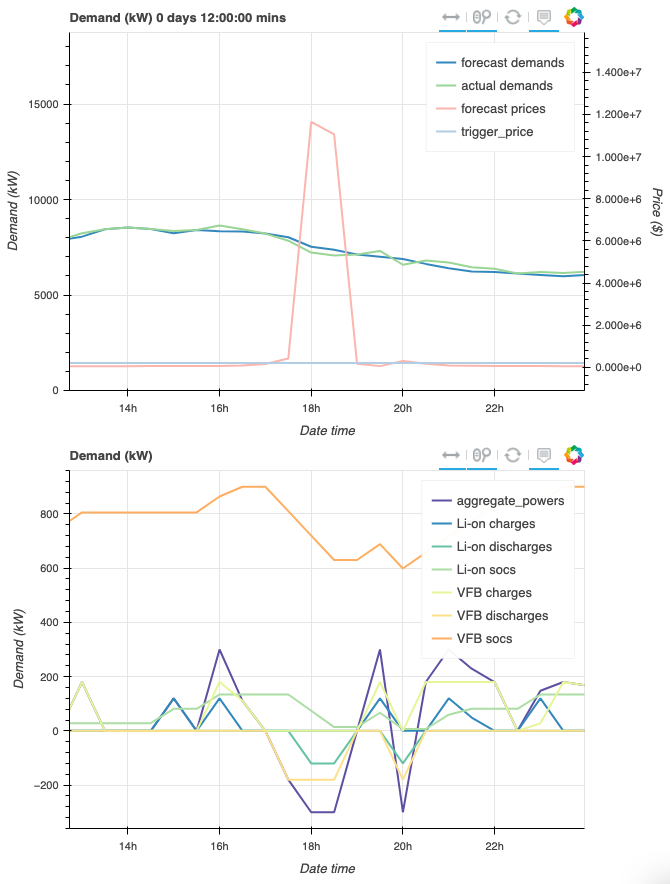
\includegraphics[width=1\linewidth]{pics/dr-demo}
	\caption{}
	\label{fig:dr-demo}
\end{figure}

\subsection{Experiment Results}

We have tested the effectiveness of our battery scheduling method for demand response using the data from 1 Jan 2020 to 30 Dec 2020 in the following step: